\documentclass{standalone}

\usepackage[american]{circuitikz}

\begin{document}
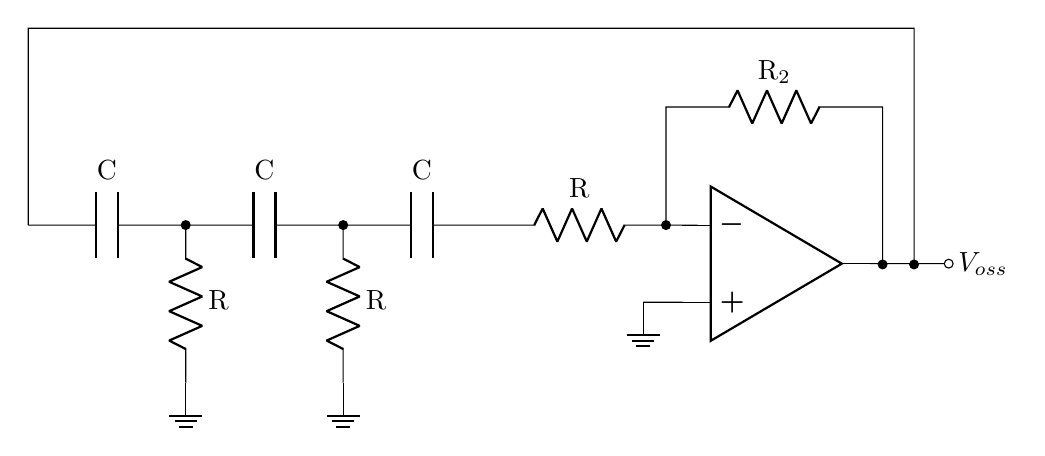
\begin{tikzpicture}
	\draw
	(0,0) to [short] ++(0, 2.5)
	to [short] ++ (11.25,0)
	to [short, -*] ++ (0, -3.0)
	(0,0) to [C, l=C] (2,0)
	to [C, l=C, *-*] (4,0)
	to [C, l=C] (6,0)
	to [R, l=R] (8,0)
	to [short] (8.5, 0)
	(8.1, 0) to [short, *-] (8.1, 1.5)
	to [R, l=R$_2$] ++(2.75, 0)
	to [short, -*] ++(0, -2)
	(2,0) to [R, l=R] (2, -2) node[ground] {}
	(4,0) to [R, l=R] (4, -2) node[ground] {}
	(9.5,-0.49) node[op amp] (opamp) {}
	(opamp.out) to [short, -o] ++(1, 0) node[right] {$V_{oss}$}
	(opamp.+) to [short] ++(-0.5, 0) node[ground] {}
	;
\end{tikzpicture}
\end{document}